Dead Link Checker\footnote{\url{https://www.deadlinkchecker.com} (Diakses pada 30 Agustus 2025)} adalah sebuah situs web yang dikembangkan oleh DLC Websites untuk mendeteksi tautan rusak pada situs web. Situs ini memiliki tiga layanan utama, yaitu \textit{site check} yang tersedia secara gratis, serta \textit{multi check} dan \textit{auto check} yang tersedia secara berbayar. Layanan \textit{site check} digunakan untuk memeriksa tautan pada satu situs web, \textit{multi check} memungkinkan pemeriksaan pada beberapa situs sekaligus, sedangkan \textit{auto check} menyediakan pemeriksaan berkala dengan laporan hasil yang dikirim melalui email.

\subsubsection*{Tampilan dan Interaksi}

Gambar~\ref{fig:analisis-deadlinkchecker} menunjukkan tampilan antarmuka Dead Link Checker pada layanan \textit{site check} saat proses pemeriksaan berlangsung. Alur penggunaan secara umum dimulai dengan memasukkan alamat situs, memilih mode pemeriksaan, lalu menekan tombol \textit{check} untuk memulai proses. Selama pemeriksaan berjalan, sistem menampilkan ringkasan progres dan hasilnya diperbarui secara langsung dalam bentuk tabel.


\begin{figure}[H]
    \centering
    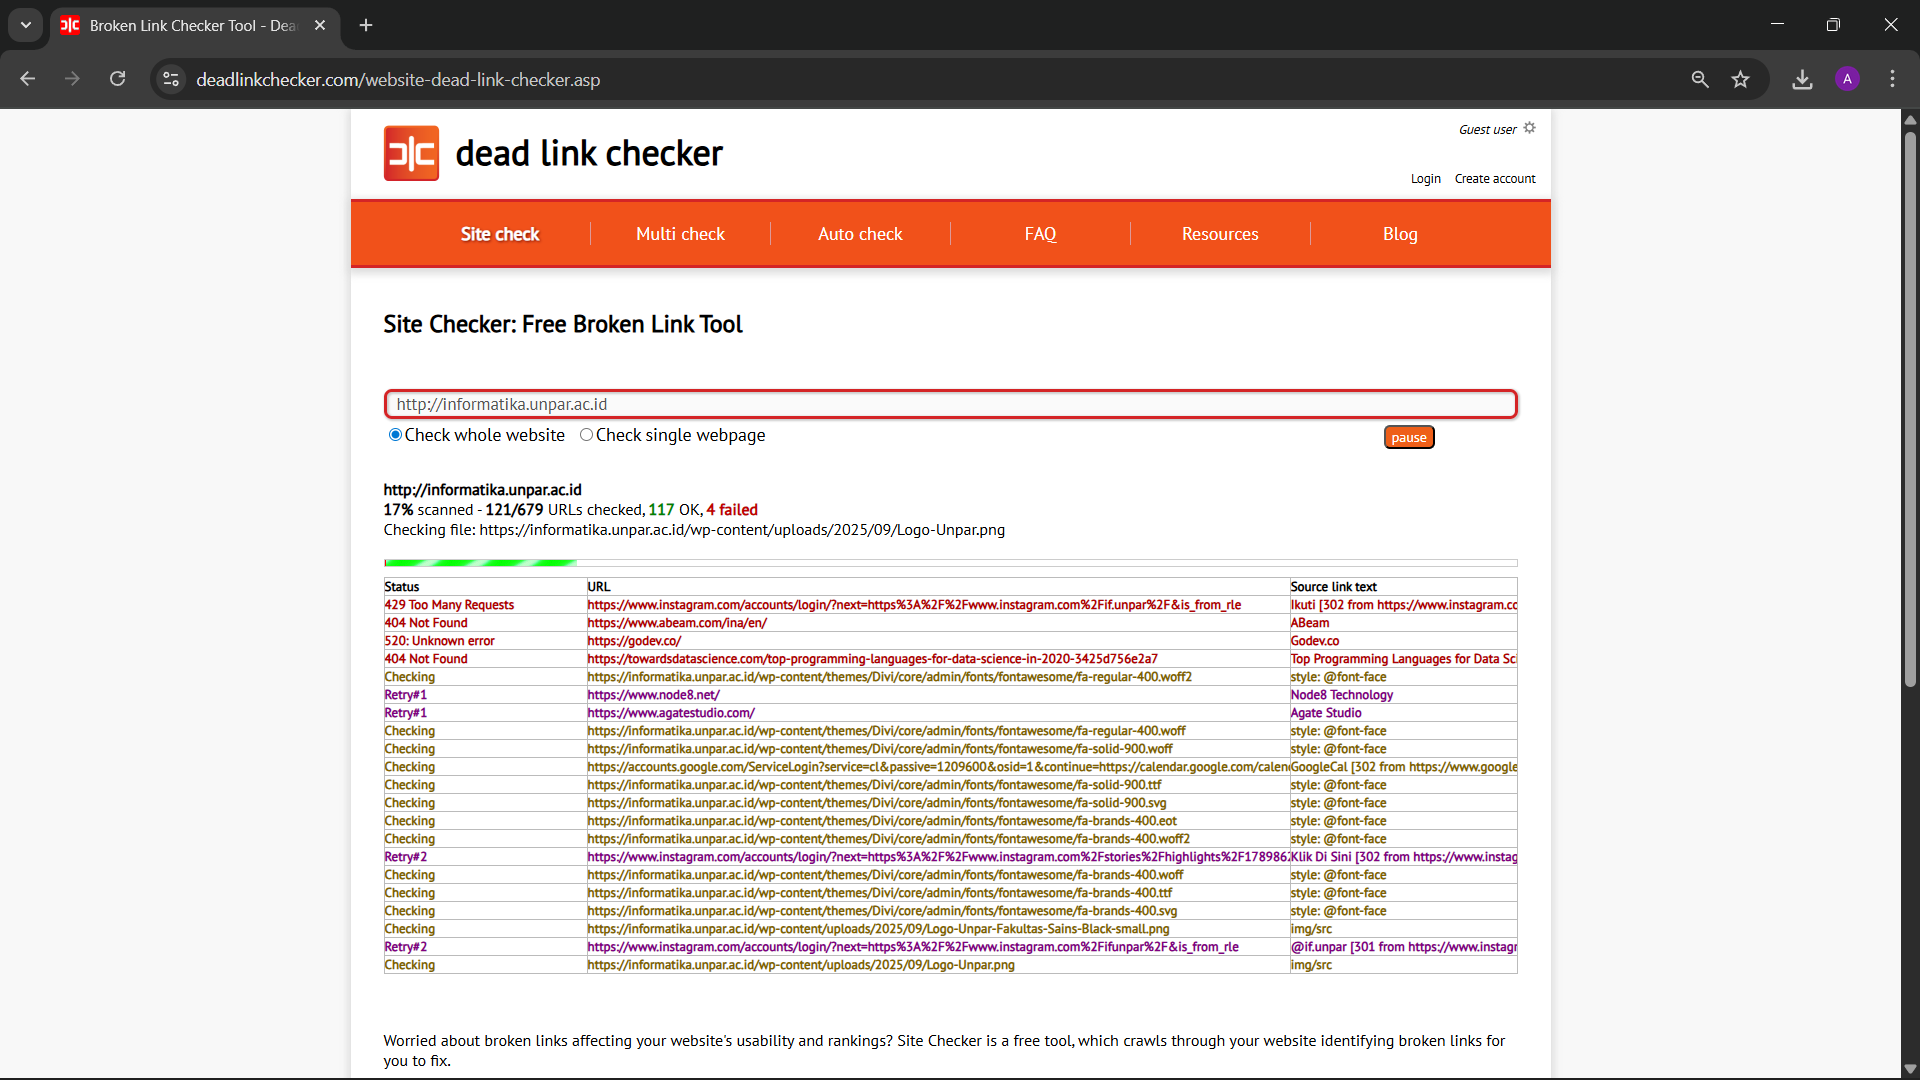
\includegraphics[width=0.9\textwidth]{Gambar/030202-dead-link-checker.png}
    \caption{Antarmuka Dead Link Checker}
    \label{fig:analisis-deadlinkchecker}
\end{figure}

Berikut adalah penjelasan komponen antarmuka pengguna pada layanan \textit{site check} :
\begin{enumerate}
    \item \textbf{Input URL}\\  
    Pengguna cukup memasukkan alamat domain atau halaman dengan URL absolut yang ingin diperiksa. Jika skema tidak dituliskan, sistem secara otomatis menambahkan awalan \texttt{http://}. Hal ini menyederhanakan input, meskipun dapat menimbulkan masalah pada situs yang hanya mendukung skema HTTPS.  

    \item \textbf{Mode pemeriksaan}\\  
    Dead Link Checker menyediakan dua opsi, yakni \textit{Check whole website} untuk menelusuri seluruh halaman dalam domain yang sama dengan URL input, dan \textit{Check single webpage} untuk memeriksa hanya halaman yang diberikan sesuai URL input.
 
    \item \textbf{Kontrol proses}\\
    Pemeriksaan tautan dijalankan dengan menekan tombol \textit{check}. Setelah proses berlangsung, tombol ini berubah menjadi \textit{pause} yang jika ditekan maka akan menghentikan sementara proses pemeriksaan dan menyimpan posisi terakhir. Pada kondisi jeda, tombol \textit{pause} akan digantikan dengan dua tombol, yaitu \textit{resume} untuk melanjutkan pemeriksaan dari titik terakhir, dan \textit{cancel} untuk membatalkan seluruh proses.

    \item \textbf{Ringkasan pemeriksaan}\\  
    Ringkasan pemeriksaan menampilkan informasi utama terkait progres yang sedang berlangsung. Bagian ini memuat alamat situs yang diperiksa, persentase pemindaian yang telah selesai, jumlah tautan yang sudah diperiksa dibandingkan dengan total tautan yang ditemukan, serta jumlah tautan yang berstatus OK dan yang \textit{failed}. Informasi tambahan juga ditampilkan berupa alamat tautan yang sedang diperiksa pada saat itu. Tepat di bawahnya terdapat \textit{progress bar} berwarna, di mana warna hijau beraksen putih menunjukkan jumlah tautan yang berstatus OK dan sedang di proses, sedangkan warna merah menunjukkan jumlah tautan yang gagal diakses.

    \item \textbf{Tabel hasil}\\
    Hasil pemeriksaan ditampilkan dalam bentuk tabel dengan tiga kolom utama yang isinya diperbarui secara langsung (\textit{real time}) selama pemeriksaan berlangsung. Tautan yang valid dihapus otomatis dari tabel setelah berhasil diperiksa, sehingga yang tersisa hanya entri yang bermasalah atau sedang diproses. Berikut adalah penjelasan untuk tiap kolom:
    \begin{itemize}
    
        \item \textbf{Status}: Pada kolom ini, awalnya semua tautan diberi status \textit{Checking}, jika pada tahap ini terjadi kegagalan koneksi atau tidak ada respons dari server, sistem secara otomatis melakukan percobaan ulang yang ditandai dengan \textit{Retry\#1} dan \textit{Retry\#2}. Apabila setelah dua kali percobaan ulang tautan tetap tidak dapat diakses, maka status akhir ditetapkan sesuai kondisi terakhir, seperti \texttt{Timeout} atau \texttt{Host not found}. Sebaliknya, jika server memberikan respons yang jelas, sistem langsung menampilkan kode hasil tanpa melakukan retry, seperti \texttt{404 Not Found}, \texttt{500 Internal Server Error}, \texttt{429 Too Many Requests}, atau kode non-standar seperti \texttt{999}. Warna latar baris juga digunakan untuk memperjelas status: kuning untuk \textit{Checking}, ungu untuk \textit{Retry}, dan merah untuk tautan yang rusak.
        
        \item \textbf{URL}: Kolom ini berisi alamat tautan yang sedang atau sudah diperiksa. Setiap entri dapat diklik untuk membuka alamat tersebut secara langsung di \textit{browser}.
        
        \item \textbf{Source link text}: Kolom ini menunjukkan teks jangkar dari tautan atau konteks halaman sumber tempat tautan ditemukan. Bagian ini juga dapat diklik untuk membuka halaman asal tautan ditemukan.
        
    \end{itemize}
\end{enumerate}

\subsubsection*{Mekanisme dan Ketentuan Teknis}  
Selain fitur yang terlihat pada antarmuka, Dead Link Checker juga memiliki mekanisme dan ketentuan teknis berikut:

\begin{enumerate}
    \item \textbf{\textit{Crawling} rekursif}\\
    Dead Link Checker bekerja dengan cara \textit{crawling} halaman web secara rekursif, yaitu dengan mengikuti setiap tautan yang ditemukan untuk kemudian dipindai kembali. Proses dimulai dari URL awal, lalu setiap tautan dalam domain yang sama diperiksa dan jika valid akan diperlakukan sebagai halaman baru untuk dianalisis. Pola ini terus diulangi hingga batas kedalaman tertentu, di mana pemeriksaan penuh (\textit{full scan}) dapat menjangkau hingga sepuluh tingkat halaman. 

    \item \textbf{Kepatuhan terhadap Robots.txt}\\
    Dead Link Checker melakukan pemindaian dengan tetap menghormati aturan pada berkas \texttt{robots.txt} yang dimiliki oleh situs web target. Pada berkas ini, administrator situs dapat menentukan direktori yang tidak boleh diakses oleh crawler atau memberi jeda antar permintaan untuk mengurangi beban server. Dead Link Checker menggunakan \textit{user-agent} khusus \texttt{www.deadlinkchecker.com}, sehingga aturan yang ditulis dengan user-agent ini akan dipatuhi. Contoh aturan yang dapat ditambahkan adalah:
    
\begin{verbatim}
User-agent: www.deadlinkchecker.com
Disallow: /shoppingbasket/
Crawl-delay: 1
\end{verbatim}

    Instruksi tersebut akan mencegah \textit{crawler} mengakses direktori \texttt{/shoppingbasket/} beserta subdirektorinya, serta memaksa jeda minimal satu detik antar permintaan. Dengan mekanisme ini, pemilik situs web memiliki kendali untuk membatasi sejauh mana Dead Link Checker dapat melakukan \textit{crawling} pada situs web mereka.

\end{enumerate}
